\باب{تعددی ردعمل}
گزشتہ بابوں میں ہم \عددی{RLC} ادوار کو حل کر چکے ہیں جہاں تعدد غیر متغیر تھی۔اس باب میں تعدد تبدیل کرتے ہوئے ادوار کا ردعمل بالمقابل تعدد دیکھا جائے گا۔آئیں شروع میں سادہ ترین پرزوں کا تعددی رد عمل دیکھیں۔سادہ ترین پرزے  مزاحمت، امالہ اور برق گیر ہیں۔تعددی رد عمل دیکھتے ہوئے سائن نما اشارات زیر استعمال لائے جائیں گے۔ 

شکل \حوالہ{شکل_تعددی_مزاحمتی_ردعمل}-الف میں مزاحمت دکھایا گیا ہے۔مزاحت کی رکاوٹ درج ذیل ہے۔
\begin{align}
Z_R=R\phase{0^{\circ}}
\end{align}
یوں مزاحمت کی رکاوٹ پر تعدد \عددی{\omega} کا کوئی اثر نہیں پایا جاتا۔مزاحمت کے رکاوٹ کی حتمی قیمت \عددی{\abs{\bZ_R}} تمام تعدد پر \عددی{R} کے برابر ہے جبکہ اس کا زاویائی ہٹاو \عددی{\phase{\bZ_R}} تمام تعدد پر صفر درجے رہتا ہے۔یہ حقائق شکل \حوالہ{شکل_تعددی_مزاحمتی_ردعمل}-ب اور شکل \حوالہ{شکل_تعددی_مزاحمتی_ردعمل}-پ میں دکھائے گئے ہیں۔
\begin{figure}
\centering
\begin{subfigure}{1\textwidth}
\centering
\begin{tikzpicture}
\draw(0,0) to [short,o-]++(\x,0) to [resistor,l_={$R$}]++(0,\y) to [short,-o]++(-\x,0);
\draw[stealth-](\x/4,\y/2)--++(-\x/4,0)--++(0,-\y/8)node[below]{$\bZ_R$};
\end{tikzpicture}
\caption*{(الف) مزاحمت کی رکاوٹ۔}
\end{subfigure}
\begin{subfigure}{0.5\textwidth}
\centering
\begin{tikzpicture}
\begin{axis}[kStyleCircuitsA,name=ka,small,
,xlabel=$\omega$,ylabel=$\abs{\bZ_R}$,ytick={0.5},yticklabels={$R$},ymax=0.75,ymin=0,xmin=0,xtick=\empty]
\addplot[domain=0:3,samples=2]{0.5};
\end{axis}%
\end{tikzpicture}%
\caption*{(ب) مزاحمتی رکاوٹ کی حتمی قیمت بالمقابل تعدد۔}
\end{subfigure}%
\begin{subfigure}{0.5\textwidth}
\centering
\begin{tikzpicture}
\begin{axis}[kStyleCircuitsA,name=ka,small,
,xlabel=$\omega$,ylabel=$\phase{\bZ_R}$,ytick={0.25},yticklabels={$0^{\circ}$},ymax=0.75,ymin=0,xmin=0,xtick=\empty]
\addplot[domain=0:3,samples=2]{0.25};
\end{axis}
\end{tikzpicture}%
\caption*{(پ) مزاحمتی رکاوٹ کا زاویہ بالمقابل تعدد۔}
\end{subfigure}%
\caption{مزاحمتی رکاوٹ کا تعدد ردعمل۔}
\label{شکل_تعددی_مزاحمتی_ردعمل}
\end{figure}

امالہ گیر کو شکل \حوالہ{شکل_تعددی_امالی_ردعمل}-الف میں دکھایا گیا ہے۔امالہ گیر کی رکاوٹ درج ذیل ہے۔
\begin{align}
\bZ_L&=j\omega L=\omega L\phase{90^{\circ}}
\end{align}
اس طرح امالہ گیر کے رکاوٹ کی حتمی قیمت تعدد بڑھانے سے بڑھتی ہے۔رکاوٹ کی مقدار کا تعدد کے ساتھ راست تنابی رشتہ ہے۔
\begin{align}
\abs{\bZ_L}=\omega L
\end{align}
صفر تعدد پر امالہ گیر کی رکاوٹ \عددی{\SI{0}{\ohm}} ہو جاتی ہے اور یہ قصر دور خاصیت رکھتا ہے جبکہ لامتناہی تعدد پر رکاوٹ کی مقدار لامتناہی ہو جاتی ہے اور امالہ گیر بطور کھلا دور عمل کرتا ہے۔امالی رکاوٹ کا زاویہ تمام تعدد پر \عددی{90^{\circ}} رہتا ہے۔
\begin{align}
\phase{\bZ_L}=90^{\circ}
\end{align}
شکل \حوالہ{شکل_تعددی_امالی_ردعمل}-ب اور شکل \حوالہ{شکل_تعددی_امالی_ردعمل}-پ میں ان حقائق کو دکھایا گیا ہے۔
\begin{figure}
\centering
\begin{subfigure}{1\textwidth}
\centering
\begin{tikzpicture}
\draw(0,0) to [short,o-]++(\x,0) to [inductor,l_={$L$}]++(0,\y) to [short,-o]++(-\x,0);
\draw[stealth-](\x/4,\y/2)--++(-\x/4,0)--++(0,-\y/8)node[below]{$\bZ_L$};
\end{tikzpicture}
\caption*{(الف) امالہ گیر کی رکاوٹ۔}
\end{subfigure}
\begin{subfigure}{0.5\textwidth}
\centering
\begin{tikzpicture}
\begin{axis}[kStyleCircuitsA,name=ka,small,
,xlabel=$\omega$,ylabel=$\abs{\bZ_L}$,ytick=\empty,ymin=0,xmin=0,xtick=\empty]
\addplot[domain=0:10,samples=10]{0.5*x};
\end{axis}%
\end{tikzpicture}%
\caption*{(ب) امالی رکاوٹ کی حتمی قیمت بالمقابل تعدد۔}
\end{subfigure}%
\begin{subfigure}{0.5\textwidth}
\centering
\begin{tikzpicture}
\begin{axis}[kStyleCircuitsA,name=ka,small,
,xlabel=$\omega$,ylabel=$\phase{\bZ_L}$,ytick={0.5},yticklabels={$90^{\circ}$},ymax=0.75,ymin=0,xmin=0,xtick=\empty]
\addplot[domain=0:3,samples=2]{0.5};
\end{axis}
\end{tikzpicture}%
\caption*{(پ) امالی رکاوٹ کا زاویہ بالمقابل تعدد۔}
\end{subfigure}%
\caption{امالی رکاوٹ کا تعدد ردعمل۔}
\label{شکل_تعددی_امالی_ردعمل}
\end{figure}

برق گیر کو شکل \حوالہ{شکل_تعددی_برق_گیری_ردعمل}-الف میں دکھایا گیا ہے۔برق گیر کی رکاوٹ درج ذیل ہے۔
\begin{align}
\bZ_C=\frac{1}{j\omega C}=\frac{1}{\omega C}\phase{-90^{\circ}}
\end{align}
اس طرح برق گیر کے رکاوٹ کی مقدار کا تعدد کے ساتھ بالعکس متناسب کا رشتہ ہے جبکہ اس کا زاویہ تمام تعدد پر \عددی{-90^{\circ}} رہتا ہے۔
\begin{align}
\abs{\bZ_C}&=\frac{1}{\omega C}\\
\phase{bZ_C}&=-90^{\circ}
\end{align}
ان تعلقات کو شکل \حوالہ{شکل_تعددی_برق_گیری_ردعمل}-ب اور شکل \حوالہ{شکل_تعددی_برق_گیری_ردعمل}-پ میں دکھایا گیا ہے۔ صفر تعدد پر برق گیر کی رکاوٹ لامتناہی ہو جاتی ہے لہٰذا یہ بطور کھلا دور عمل کرتا ہے جبکہ لامتناہی تعدد پر رکاوٹ کی مقدار صفر ہو جاتی ہے اور یہ قصر دور کردار ادا کرتا ہے۔
\begin{figure}
\centering
\begin{subfigure}{1\textwidth}
\centering
\begin{tikzpicture}
\draw(0,0) to [short,o-]++(\x,0) to [capacitor,l_={$C$}]++(0,\y) to [short,-o]++(-\x,0);
\draw[stealth-](\x/4,\y/2)--++(-\x/4,0)--++(0,-\y/8)node[below]{$\bZ_C$};
\end{tikzpicture}
\caption*{(الف) برق گیر کی رکاوٹ۔}
\end{subfigure}
\begin{subfigure}{0.5\textwidth}
\centering
\begin{tikzpicture}
\begin{axis}[kStyleCircuitsA,name=ka,small,
,xlabel=$\omega$,ylabel=$\abs{\bZ_C}$,ytick=\empty,ymin=0,xmin=0,xtick=\empty]
\addplot[domain=10:60,samples=100]{1/(0.5*x)};
\end{axis}%
\end{tikzpicture}%
\caption*{(ب) برق گیر رکاوٹ کی حتمی قیمت بالمقابل تعدد۔}
\end{subfigure}%
\begin{subfigure}{0.5\textwidth}
\centering
\begin{tikzpicture}
\begin{axis}[kStyleCircuitsA,name=ka,small,
,xlabel=$\omega$,ylabel=$\phase{\bZ_C}$,ytick={0.5},yticklabels={$-90^{\circ}$},ymax=0.75,xmin=0,xtick=\empty]
\addplot[domain=0:3,samples=2]{0.5};
\end{axis}
\end{tikzpicture}%
\caption*{(پ) برق گیر رکاوٹ کا زاویہ بالمقابل تعدد۔}
\end{subfigure}%
\caption{برق گیر رکاوٹ کا تعدد ردعمل۔}
\label{شکل_تعددی_برق_گیری_ردعمل}
\end{figure}

سادہ ترین پرزوں کو نپٹانے کے بعد ذرہ مشکل ادوار دیکھتے ہیں۔شکل میں مزاحمت، امالہ گیر اور برق گیر سلسلہ وار جڑے دکھائے گئے ہیں۔ان کی کل رکاوٹ \عددی{\bZ_s} لکھتے ہیں
\begin{align*}
\bZ_s&=\bZ_R+\bZ_L+\bZ_C\\
&=R+j\omega L+\frac{1}{j\omega C}\\
&=R+j\left(\omega L-\frac{1}{\omega C}\right)
\end{align*}
اس تفاعل کو شکل \حوالہ{شکل_تعددی_مزاحمت_املہ_برق_گیر_سلسلہ_وار_ردعمل}-ب اور شکل \حوالہ{شکل_تعددی_مزاحمت_املہ_برق_گیر_سلسلہ_وار_ردعمل}-پ میں دکھایا گیا ہے۔
%
\begin{figure}
\centering
\begin{subfigure}{1\textwidth}
\centering
\begin{tikzpicture}
\draw(0,0) to [resistor,o-,l={$R$}]++(\x,0) to [inductor,l={$L$}]++(\x,0) to  [capacitor,l={$C$}]++(0,-\y) to [short,-o]++(-2*\x,0);
\draw[stealth-](\x/4,-\y/2)--++(-\x/4,0)--++(0,-\y/8)node[below]{$\bZ_s$};
\end{tikzpicture}
\caption*{(الف) سلسلہ وار دور۔}
\end{subfigure}
\begin{subfigure}{0.5\textwidth}
\centering
\begin{tikzpicture}
\begin{axis}[kStyleCircuitsA,name=ka,small,
,xlabel=$\omega$,ylabel=$\abs{\bZ_C}$,ytick=\empty,ymin=0,xmin=0,xtick={1},xticklabels={$\omega_0$}]
\addplot[domain=0:5,samples=100]{sqrt((1-x^2)^2+x^2)/x};
\end{axis}%
\end{tikzpicture}%
\caption*{(ب) مقدار بالمقابل تعدد۔}
\end{subfigure}%
\begin{subfigure}{0.5\textwidth}
\centering
\begin{tikzpicture}
\begin{axis}[kStyleCircuitsA,name=ka,small,
,xlabel=$\omega$,ylabel=$\phase{\bZ_C}$,ytick={-90,0,90},yticklabels={$-90^{\circ}$,$0^{\circ}$,$90^{\circ}$},ymax=120,xmin=0,xtick={1},xticklabels={$\omega_0$}]
\addplot[domain=0.01:3,samples=100]{atan(x-1/x)};
\end{axis}
\end{tikzpicture}%
\caption*{(پ) زاویہ بالمقابل تعدد۔}
\end{subfigure}%
\caption{سلسلہ وار جڑے مزاحمت، امالہ گیر اور برق گیر کا تعدد ردعمل۔}
\label{شکل_تعددی_مزاحمت_املہ_برق_گیر_سلسلہ_وار_ردعمل}
\end{figure}
%======================
\ابتدا{مثال}\شناخت{مثال_تعددی_بوڈا_خط_مزاحمت_امالہ_برق_گیر_رو_الف}
شکل \حوالہ{شکل_تعددی_بوڈا_خط_مزاحمت_امالہ_برق_گیر_رو_الف}-الف میں دیے دور کی رو کے مقدار بالمقابل تعدد اور زاویہ بالمقابل تعدد کے خط کھینچیں۔
\begin{figure}
\centering
\begin{subfigure}{1\textwidth}
\centering
\begin{tikzpicture}
\draw(0,0) to [resistor,l={$\SI{10}{\ohm}$}]++(\x,0) to [inductor,l={$\SI{0.15}{\henry}$}]++(\x,0) to  [capacitor,l={$\SI{4}{\milli\farad}$}]++(0,-\y) to [short]++(-2*\x,0) to [american voltage source,l={$20\phase{0^{\circ}}\,\si{\volt}$}]++(0,\y);
\end{tikzpicture}
\caption*{(الف)}
\end{subfigure}
\begin{subfigure}{1\textwidth}
\centering
\begin{tikzpicture}
\node[anchor=south west,inner sep=0] (image) at (0,0) {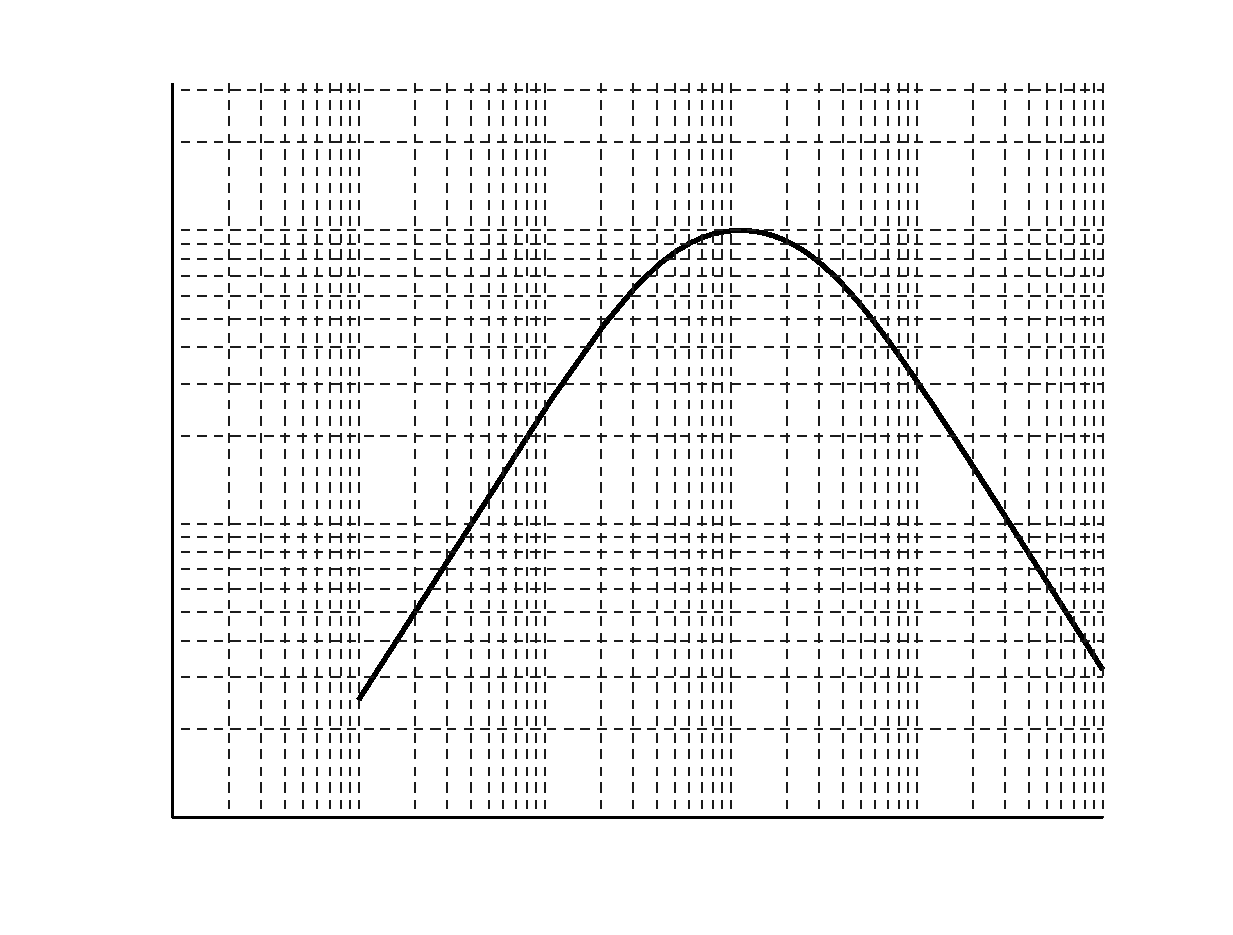
\includegraphics[height=3cm,width=7cm]{bodeMagnitudeRLC}};
\begin{scope}[x={(image.south east)},y={(image.north west)}]
%	\draw[help lines,xstep=.1,ystep=.1] (0,0) grid (1,1);
%	\foreach \x in {0,1,...,9} { \node [anchor=north] at (\x/10,0) {0.\x}; }
%	\foreach \y in {0,1,...,9} { \node [anchor=east] at (0,\y/10) {0.\y}; }
%
\draw(0.28,0.1)node[below]{$10^{-1}$};
\draw(0.45,0.1)node[below]{$10^{0}$};
\draw(0.6,0.1)node[below]{$10^{1}$};
\draw(0.75,0.1)node[below]{$10^{2}$};
\draw(0.9,0.1)node[below]{$f(\si{\hertz})$};
%
\draw(0.14,0.76)node[left]{$10^2$};
\draw(0.14,0.45)node[left]{$10^1$};
\draw(0.14,0.12)node[left]{$10^{-1}$};
\draw(0,0.45)node[left]{مقدار};
\end{scope}
\end{tikzpicture}
\caption*{(ب)}
\end{subfigure}
\caption{مثال \حوالہ{مثال_تعددی_بوڈا_خط_مزاحمت_امالہ_برق_گیر_رو_الف} کا دور۔}
\label{شکل_تعددی_بوڈا_خط_مزاحمت_امالہ_برق_گیر_رو_الف}
\end{figure}
%

\انتہا{مثال}
%========================
